\section{Views in Oracle 12c}
\phantomsection

Oracle presents a very similar way to treats views in 12c, we have the same functions for creating, updating and deleting a view, but it comes with an addition of different parameters specification. OR REPLACE, INSTEAD OF, UNUSABLE are just a small part of triggers defined on a conventional view.\\
To create a View in PL/SQL we use the same implementation as we did with TSQL, using CREATE VIEW command:\\
\lstinputlisting[style=mystyle, language=SQL, caption={Views creating statements},]{sourcecode/Create_View_Oracle.sql}

Different views are created with different purposes, based on what are our needs for the specific task, table or interaction with the database.\\
We can create a single table view or or multi-table view, with functions in the WHERE or SELECT clause, but much more of that, we can create Force Views and Parameterized Views.

\textbf{Force View} allows us to create a view even if it is invalid.\\
\lstinputlisting[style=mystyle, language=SQL, caption={Views creating statements},]{sourcecode/Create_Force_View_Oracle.sql}

\textbf{Parameterized View} are a type of views with a filter or function in WHERE clause or SELECT clause.\\
\lstinputlisting[style=mystyle, language=SQL, caption={Views creating statements},]{sourcecode/Create_Parameter_View_Oracle.sql}

Oracle allows us to do such options as altering a view and commenting views or column views. It can be done easily with ALTER VIEW <view name> COMPILE and 
COMMENT ON TABLE <table name> IS '<comment string>';\\
With \textbf{View Update} there are also tricks and a set of restrictions that a view can not include in order to be updated. Such constraints are:
• Set Operators (INTERSECT, MINUS, UNION, UNION ALL)
• DISTINCT
• Group Aggregate Functions (AVG, COUNT, MAX, MIN, SUM, etc.)
• GROUP BY Clause
• ORDER BY Clause
• CONNECT BY Clause
• START WITH Clause
• Collection Expression In A Select List
• Subquery In A Select List
• Join Query\\

In order to update a view we have to take into account those constraints at the stage of view creation and try to complete them in order to update the view later. \\
\\

\textbf{Deleting a view} in Oracle 12c is made the same as in Microsoft SQL Server, with Drop operation.
\lstinputlisting[style=mystyle, language=SQL, caption={Views creating statements},]{sourcecode/Drop_View_Oracle.sql}

Interesting thing about views is that even if the base table was deleted the view will continue to exist however if we will try to query the Oracle VIEW we will receive a message indicating that the Oracle VIEW has errors.\\
\\
\textbf{Materialized Views:}\\
Originally called snapshots, materialized views were introduced in Oracle8i and are only available in the Enterprise Edition. Like a regular view, the data in a materialized view results from a query. However, the results of a regular view are transitory—they are lost once the query is complete and, if needed again, the query must be re-executed. In contrast, the results from a materialized view are kept and physically stored in a database object that resembles a table. This feature means that the underlying query only needs to be executed once and then the results are available to all who need them.

Oracle Database 12c allows for synchronous refreshes of the materialized views when configured to use a refresh method besides manual or on-demand. It utilizes partitioning and dependencies between the objects to minimize the time it takes to refresh and maintain the data as close to the underlying tables as possible.
Materialized views are used as a performance-enhancing technique. In this section, you learn about the following uses of these views, as they are applicable to the topic of large databases.

Performing data summarization (for example, sums and averages)
Prejoining tables
Performing CPU-intensive calculations
Replicating and distributing data
In large databases, particularly data warehousing environments, there is always a need to summarize, join, perform calculations, or do all three operations at once on large numbers of records for the purposes of reporting and analysis. To improve performance in the past, a combination of views and physical tables were usually implemented that contained the results of these operations. The summary tables would require some type of extraction, transformation, and load (ETL) process to populate and refresh them. In addition to the base tables containing the detailed data, the users would need to know which combinations of the views and/or summary tables to use. 

Using materialized views has several advantages over more traditional methods. These include the following:

• Materialized views have a built-in data refresh process, which can provide an automatic update or repopulation of a materialized view without any programming on the part of the DBA.\\
• As mentioned earlier, the data in materialized views can be partitioned, using the same techniques that apply to tables.\\
• Materialized views are transparent to the users. This is probably the most attractive feature of using materialized views. We expand more on this in the next section when we discuss automatic query rewriting.\\
\begin{figure}[ht!]
    \centering
    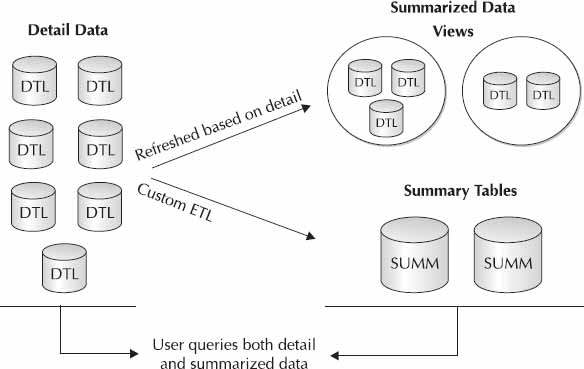
\includegraphics[width=0.5\textwidth]{FIG1}
    \caption{Summarization using views and summary tables}
    \label{fig_21}
\end{figure}
\\
\begin{figure}[ht!]
    \centering
    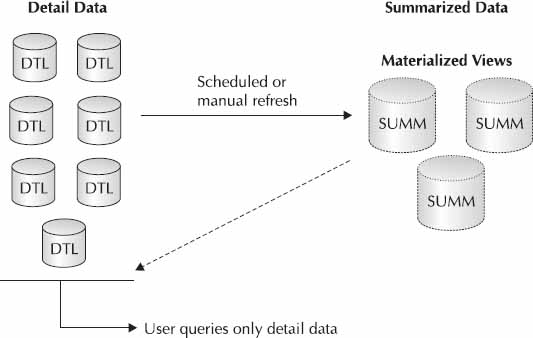
\includegraphics[width=0.5\textwidth]{FIG2}
    \caption{Summarization using materialized views}
    \label{fig_21}
\end{figure}
At this point, you may be asking yourself: “How do I determine what materialized views to create and at what level of summarization?” Oracle Database 12c has some utilities to help. These utilities are collectively called the SQL Tuning Advisor and will recommend materialized views based on historical queries, or based on theoretical scenarios. They can be run from the Oracle Enterprise Manager (OEM) Grid Control, or by calling the dbms advisor package.
\clearpage